\documentclass[11pt]{article}
\pdfinfoomitdate=1
\pdftrailerid{}
\pdfsuppressptexinfo=15
\usepackage[T1]{fontenc}
\usepackage{lmodern,microtype,amsmath,amssymb,amsthm,mathtools}
\usepackage[margin=1in]{geometry}
\usepackage{tikz}
\usetikzlibrary{arrows.meta}
\PassOptionsToPackage{hyphens}{url}
\usepackage[colorlinks=true,linkcolor=blue!45!black,citecolor=blue!45!black,urlcolor=blue!45!black]{hyperref}
\input{glyphtounicode}
\pdfglyphtounicode{angbracketleftBigg}{27E8}
\pdfglyphtounicode{angbracketleftbig}{27E8}
\pdfglyphtounicode{angbracketrightBigg}{27E9}
\pdfglyphtounicode{angbracketrightbig}{27E9}
\pdfglyphtounicode{arrowhookleft}{02D3}
\pdfglyphtounicode{axisshort}{002D}
\pdfglyphtounicode{arrowaxisright}{2192}
\pdfglyphtounicode{circleplusdisplay}{2A01}
\pdfglyphtounicode{braceex}{23AA}
\pdfglyphtounicode{braceleftbigg}{007B}
\pdfglyphtounicode{braceleftbt}{23A9}
\pdfglyphtounicode{braceleftmid}{23A8}
\pdfglyphtounicode{bracelefttp}{23A7}
\pdfglyphtounicode{bracerightbigg}{007D}
\pdfglyphtounicode{bracketleftbig}{005B}
\pdfglyphtounicode{bracketleftbigg}{005B}
\pdfglyphtounicode{bracketleftbt}{23A3}
\pdfglyphtounicode{bracketlefttp}{23A1}
\pdfglyphtounicode{bracketrightbig}{005D}
\pdfglyphtounicode{bracketrightbigg}{005D}
\pdfglyphtounicode{bracketrightbt}{23A6}
\pdfglyphtounicode{bracketrighttp}{23A4}
\pdfglyphtounicode{hatwide}{0302}
\pdfglyphtounicode{hatwider}{0302}
\pdfglyphtounicode{hatwidest}{0302}
\pdfglyphtounicode{integraldisplay}{222B}
\pdfglyphtounicode{integraltext}{222B}
\pdfglyphtounicode{intersectiondisplay}{22C2}
\pdfglyphtounicode{intersectiontext}{22C2}
\pdfglyphtounicode{mapsto}{007C}
\pdfglyphtounicode{parenleftBig}{0028}
\pdfglyphtounicode{parenleftBigg}{0028}
\pdfglyphtounicode{parenleftbig}{0028}
\pdfglyphtounicode{parenleftbigg}{0028}
\pdfglyphtounicode{parenleftbt}{239D}
\pdfglyphtounicode{parenlefttp}{239B}
\pdfglyphtounicode{parenrightBig}{0029}
\pdfglyphtounicode{parenrightBigg}{0029}
\pdfglyphtounicode{parenrightbig}{0029}
\pdfglyphtounicode{parenrightbigg}{0029}
\pdfglyphtounicode{parenrightbt}{23A0}
\pdfglyphtounicode{parenrighttp}{239E}
\pdfglyphtounicode{productdisplay}{220F}
\pdfglyphtounicode{producttext}{220F}
\pdfglyphtounicode{radicalbig}{221A}
\pdfglyphtounicode{radicalbigg}{221A}
\pdfglyphtounicode{radicalBigg}{221A}
\pdfglyphtounicode{floorleftbigg}{230A}
\pdfglyphtounicode{floorrightbigg}{230B}
\pdfglyphtounicode{floorleftBigg}{230A}
\pdfglyphtounicode{floorrightBigg}{230B}
\pdfglyphtounicode{ceilingleftBig}{2308}
\pdfglyphtounicode{ceilingrightBig}{2309}
\pdfglyphtounicode{summationdisplay}{2211}
\pdfglyphtounicode{summationtext}{2211}
\pdfglyphtounicode{uniontext}{22C3}
\pdfglyphtounicode{vextenddouble}{2225}
\pdfglyphtounicode{vextendsingle}{007C}
\pdfglyphtounicode{tildewide}{0303}
\pdfglyphtounicode{tildewider}{0303}
\pdfglyphtounicode{bracketleftBigg}{005B}
\pdfglyphtounicode{bracketrightBigg}{005D}
\pdfglyphtounicode{braceleftBigg}{007B}
\pdfglyphtounicode{bracerightBigg}{007D}
\pdfglyphtounicode{braceleftBig}{007B}
\pdfglyphtounicode{bracerightBig}{007D}
\pdfglyphtounicode{coproductdisplay}{2210}
\pdfglyphtounicode{bracketleftBig}{005B}
\pdfglyphtounicode{bracketrightBig}{005D}
\pdfglyphtounicode{radicalBig}{221A}
\pdfglyphtounicode{uniondisplay}{22C3}
\pdfglyphtounicode{logicalandtext}{22C0}
\pdfglyphtounicode{logicalanddisplay}{22C0}
\pdfglyphtounicode{circlemultiplytext}{2A02}
\pdfglyphtounicode{circlemultiplydisplay}{2A02}
\pdfglyphtounicode{braceleftbig}{007B}
\pdfglyphtounicode{bracerightbig}{007D}
\pdfglyphtounicode{bracerighttp}{23AB}
\pdfglyphtounicode{bracerightmid}{23AC}
\pdfglyphtounicode{bracerightbt}{23AD}
\pdfgentounicode=1

\newcommand{\FieldImportLocator}{Lemma~3.1}
\newcommand{\CommutantImportLocator}{Lemma~1.2}

\hypersetup{pdftitle={Backward intertwiners and a transitive commutant},pdfauthor={OpenAI}}
\newtheorem{theorem}{Theorem}[section]
\newtheorem{lemma}[theorem]{Lemma}
\newtheorem{proposition}[theorem]{Proposition}
\newtheorem{corollary}[theorem]{Corollary}
\theoremstyle{remark}\newtheorem{remark}[theorem]{Remark}
\DeclareMathOperator{\Lat}{Lat}
\DeclareMathOperator{\ran}{ran}
\newcommand{\B}{\mathcal B}
\newcommand{\Z}{\mathbb Z}
\newcommand{\C}{\mathbb C}
\newcommand{\A}{\mathcal A}
\newcommand{\Ktail}[1]{K_{\ge #1}}
\newcommand{\norm}[1]{\lVert #1\rVert}
\title{Backward intertwiners and a transitive commutant}
\author{OpenAI}
\date{September 27, 2026}
\begin{document}
\maketitle
\begin{abstract}
We give a negative answer to the hyperinvariant-subspace problem by
constructing, on every infinite-dimensional separable complex Hilbert space,
a nonzero bounded norm-quasinilpotent operator with no nonzero proper closed
hyperinvariant subspace. Its commutant is a proper strongly closed unital
transitive complex operator algebra.
\end{abstract}
\tableofcontents
\section{Introduction}
Let $H$ be a complex Hilbert space and let $\B(H)$ denote its bounded
linear operators. The \emph{commutant} of $S\in\B(H)$ is
\[
 \{S\}'=\{A\in\B(H):AS=SA\}.
\]
A closed subspace is \emph{hyperinvariant} for $S$ if every operator in
$\{S\}'$ leaves it invariant. An operator algebra is \emph{transitive}
if its only closed common invariant subspaces are $\{0\}$ and $H$.
Thus $S$ has no nonzero proper closed hyperinvariant subspace precisely
when its commutant is transitive.

The hyperinvariant-subspace problem asks whether every bounded nonscalar
operator on an infinite-dimensional separable complex Hilbert space has
a nonzero proper closed hyperinvariant subspace. The construction below
gives a negative answer. Its purpose is to exhibit the mechanism
explicitly: the ordinary invariant subspaces of each weighted-shift
fiber are coordinate tails, and a second, commuting operator moves those
tails backward. Invariance under the commutant therefore imposes a
strict descent that cannot persist on a probability space.

\subsection{The construction theorem}
Put $K=\ell^2(\Z)$, with orthonormal basis $(e_j)_{j\in\Z}$, and define
\[
 \Ktail{h}=\overline{\operatorname{span}}\{e_j:j\ge h\}
 \quad(h\in\Z),\qquad
 \Ktail{-\infty}=K,\qquad \Ktail{+\infty}=\{0\}.
\]
Let $X=\Z_2$ be the compact additive group of $2$-adic integers, the
inverse limit of the groups $\Z/2^m\Z$. Equip it with completed Haar
probability $\mu$, put $\theta x=x+1$, and set $H_0=L^2(X,\mu;K)$.
For $g\in L^\infty(X)$, the scalar multiplier is
$(M_gf)(x)=g(x)f(x)$.

\begin{theorem}\label{thm:direct-model}
There are measurable positive weights $\beta_j:X\to(0,\infty)$,
$j\in\Z$, and a contraction $V\in\B(H_0)$ with the following properties.
The shifts
\[
 S_xe_j=\beta_j(x)e_{j+1},\qquad (Sf)(x)=S_xf(x),
\]
define a bounded operator $S$ on $H_0$, and:
\begin{enumerate}
\item For every $x\in X$, the closed invariant subspaces of $S_x$ are
exactly $\Ktail{h}$, $h\in\Z\cup\{-\infty,+\infty\}$.
\item The operator $S$ is nonzero, $\|S\|=e^{-10}$, and for every
integer $n\ge1$,
\begin{equation}\label{eq:main-power-bound}
 \|S^n\|\le
 \exp\left(-10\left\lfloor\frac{(n+1)^2}{4}\right\rfloor\right).
\end{equation}
\item The operator $V$ commutes with $S$ and has the form
\[
 (Vf)(\theta x)=V_xf(x),\qquad V_xe_j=b_j(x)e_{j-1},
\]
where $0\le b_j(x)\le1$ are measurable and are positive on a common
conull set. On that set,
\[
 \overline{V_x\Ktail{h}}=\Ktail{h-1}\quad(h\in\Z),
 \qquad \overline{V_xK}=K.
\]
\item The unital complex algebra generated by $S$, $V$, and all
scalar multipliers $M_g$ is transitive.
\end{enumerate}
\end{theorem}

All generators in the last assertion commute with $S$. The explicit
power bound implies norm-quasinilpotence,
$\lim_{n\to\infty}\|S^n\|^{1/n}=0$, while the first assertion will give
many ordinary invariant subspaces of the resulting operator.

\begin{corollary}\label{cor:direct-algebra}
Every infinite-dimensional separable complex Hilbert space admits a
nonzero bounded norm-quasinilpotent operator with no nonzero proper
closed hyperinvariant subspace. Its commutant is a proper strongly
closed unital transitive complex operator algebra.
\end{corollary}

Here the strong operator topology is pointwise norm convergence on
$H$. Consequently the commutant in the corollary also gives a negative
answer to the question whether every unital transitive operator algebra
is strongly dense in $\B(H)$.

\subsection{Context and relation to the companion}
Douglas and Pearcy studied the connection between hyperinvariant
subspaces and transitive algebras~\cite{DouglasPearcy1972}. A major
positive result is Arveson's density theorem: a transitive algebra on
a separable Hilbert space which contains a maximal abelian self-adjoint
subalgebra of $\B(H)$ is strongly dense in $\B(H)$
\cite[Theorem~3.3]{Arveson1967}. The scalar multiplier algebra used here
has infinite multiplicity. Section~\ref{sec:structure} gives an explicit
operator commuting with every such multiplier that is not itself a
scalar multiplier, so the maximality hypothesis is absent.

Domar's work on invariant subspaces of weighted translation spaces
\cite{Domar1981} and Grabiner's work on unicellular shifts
\cite{Grabiner1982} provide the classical lattice ideas behind the
fibers. Section~\ref{sec:criterion} proves the precise quadratic
weighted-translation criterion we need. Its convex-envelope and
support-separation argument follows Domar's method. The proof includes
both normalized convolution-tail estimates; no general criterion for
arbitrary weights is assumed. Our additional task is to link the fibers
by a bounded commuting operator that moves their invariant tails
backward. Opposite logarithmic changes at the two ends of the bilateral
sequence make this possible, and one measurable normalization controls
the operator over the whole base.

Atzmon and Sodin constructed completely indecomposable bilateral
weighted shifts with spectrum the unit circle~\cite{AtzmonSodin1999};
their 1999 paper left open whether those shifts have proper hyperinvariant
subspaces. Here the extra commutant action is supplied by transport
between different fibers. For a study of operators with shift-type invariant subspaces,
see K\'erchy~\cite{Kerchy2026}.
The invariant- and hyperinvariant-subspace problems must remain
distinct: the K\'erchy--Pearcy preprint claiming an equivalence was
withdrawn after a counterexample to its Theorem~3
\cite{KerchyPearcy2025Withdrawn}. The operator constructed here preserves
every fixed tail $L^2(X;\Ktail{h})$; its hyperinvariant conclusion is
proved directly.

The companion paper \cite{CircleCompanion} constructs, for every
prescribed irrational rotation, a continuous circle weight whose
operator in the rotation factor has no nontrivial invariant projection
in that factor. It derives the existence conclusion of
Corollary~\ref{cor:direct-algebra} by the usual projection argument;
see also Dykema~\cite[Proposition~2.1]{Dykema2005}.
The present construction has a different purpose: it exhibits the
ordinary invariant tails, the bounded operator that moves them backward,
and the explicit estimate~\eqref{eq:main-power-bound}. The two proofs
use different constructions. Our only proof imports from the companion
are the two elementary facts stated below.

\subsection{Proof overview and elementary inputs}
The proof first makes the possible fiber subspaces completely explicit.
Section~\ref{sec:criterion} classifies invariant subspaces of a weighted
translation whose logarithmic weights have opposite quadratic growth
at the two ends. Section~\ref{sec:fibers} constructs weights over
$\Z_2$ satisfying that criterion in every fiber. Their decay also gives
the uniform power estimate, which proves norm-quasinilpotence of the
operator on $H_0$ rather than merely of its individual fibers.

To couple the fibers, we prescribe a map from $e_j$ at $x$ to a positive
multiple of $e_{j-1}$ at $\theta x$. Commutation with the forward shifts
determines a recurrence for those multiples. Section~\ref{sec:intertwiner}
solves the recurrence in both directions. The logarithmic changes of the
weights under $\theta$ have opposite signs at the two ends; the
coefficients therefore decay in both directions. Dividing all coefficients in each fiber by their common
supremum yields the contraction $V$ without changing commutation.

Finally, a subspace invariant under every scalar multiplier has an
orthogonal projection represented by a measurable projection field.
Invariance under $S$ makes each fiber a tail $\Ktail{s(x)}$.
Section~\ref{sec:subspaces} uses the dense images under $V_x$ to obtain
\[
 s(\theta x)\le s(x)-1\qquad\text{whenever }s(x)\in\Z.
\]
Probability preservation excludes finite labels, and ergodicity excludes
a nonconstant mixture of full and zero fibers. Section~\ref{sec:structure}
then proves the corollary and records the structure of the example.

We use the following two elementary inputs, with the stated scope.
Their complete proofs are in the companion \cite{CircleCompanion}.
\begin{enumerate}
\item \emph{Fields from scalar multipliers}
\cite[\FieldImportLocator]{CircleCompanion}.
For a probability space $(Y,\nu)$, $K=\ell^2(\Z)$, and
$A\in\B(L^2(Y;K))$ commuting with every scalar multiplier,
there is an essentially bounded field $A_y\in\B(K)$, unique almost
everywhere, such that
\[
 (Af)(y)=A_yf(y),\qquad \|A_y\|\le\|A\|\quad\text{a.e.}
\]
For every $v\in K$, the map $y\mapsto A_yv$ is measurable.
Products and adjoints act fiberwise; an orthogonal projection has
orthogonal projection fibers outside one null set.
\item \emph{The commutant algebra}
\cite[\CommutantImportLocator]{CircleCompanion}.
For any bounded nonscalar operator on a complex Hilbert space, its
commutant is a proper strongly closed unital complex algebra. If its
only closed common invariant subspaces are zero and the whole space,
that algebra is transitive.
\end{enumerate}
The first input requires no base transformation, covariance, trace or
factor assumption. We apply it only after proving reduction by all
scalar multipliers. The second requires neither separability nor
quasinilpotence; the constructed operator will satisfy its nonscalarity
hypothesis. The field input is used in Section~\ref{sec:subspaces}, and the
commutant input in Section~\ref{sec:structure}.

\section{The quadratic weighted-translation criterion}\label{sec:criterion}
We first prove a criterion that makes every invariant fiber subspace a coordinate tail. The proof concerns one weighted sequence and does not involve the base transformation.

For a positive sequence $w=(w_j)_{j\in\Z}$, set
\[
 \ell^2(w)=\left\{z:\sum_{j\in\Z}|w_jz_j|^2<\infty\right\},
 \qquad \norm{z}_{\ell^2(w)}^2=\sum_{j\in\Z}|w_jz_j|^2.
\]
If $w$ is decreasing, right translation $(Rz)_j=z_{j-1}$ is a contraction on this space. For a sequence $q_j$ on an integer interval, convexity means that $q_{j+1}-q_j$ is nondecreasing wherever the differences are defined; concavity means the reverse.

\begin{lemma}[Weighted translation criterion]\label{lem:domar}
Let $w=(w_j)_{j\in\Z}$ be positive and decreasing. Suppose that $\log w_j$ is convex for $j\le0$ and concave for $j\ge0$, that
\begin{equation}\label{eq:root-sum}
 \sum_{j\ne0}w_j^{1/j}<\infty,
\end{equation}
and that, for some $a>\log3$,
\begin{equation}\label{eq:quadratic}
 \lim_{n\to\infty}\frac{\log w_n}{n^2}=-a,
 \qquad
 \lim_{n\to\infty}\frac{\log w_{-n}}{n^2}=a.
\end{equation}
Then the closed $R$-invariant subspaces of $\ell^2(w)$ are precisely
\[
 \{z:z_j=0\text{ for }j<h\},\qquad h\in\Z\cup\{-\infty,+\infty\}.
\]
Consequently the shift $Te_j=(w_{j+1}/w_j)e_{j+1}$ on $K$ has invariant lattice $\{\Ktail{h}:h\in\Z\cup\{-\infty,+\infty\}\}$.
\end{lemma}

The convex-envelope and support-separation argument below follows the
method of Domar's weighted-translation work \cite[Section~3]{Domar1981}.
We prove the stated quadratic specialization in full, including the
normalized estimates for both convolution tails.
The signed exponent for a negative index is essential: the corresponding
summand is $w_{-n}^{-1/n}$ for $n>0$.
\begin{proof}
Multiplying the weight by a constant, assume $w_0=1$. Put
$P_n=\log w_{-n}$ and $Q_n=-\log w_n$ for $n\geq0$.
These sequences are convex, vanish at zero, and grow quadratically.
For either sequence $G=P,Q$, convexity gives
$G_n-G_{n-1}\geq G_n/n$. Put $\beta_j=w_{j+1}/w_j$. For $n\geq1$,
\[
 \beta_{-n}=e^{-(P_n-P_{n-1})}\leq w_{-n}^{-1/n},\qquad
 \beta_{n-1}=e^{-(Q_n-Q_{n-1})}\leq w_n^{1/n},
\]
The signed-root sum therefore gives
\begin{equation}\label{eq:p3-ratio-sum}
 \beta_j\leq1,
 \qquad \sum_{j\in\mathbb Z}\beta_j<\infty.
\end{equation}
In particular, $R$ is bounded. If $|c_j|w_j\leq1$ and
$|b_j|/w_j\leq1$, then for each integer $r\geq1$,
\[
 \sum_j|b_jc_{j-r}|
 \leq\sum_j\frac{w_j}{w_{j-r}}
 \leq\sum_j\beta_{j-r}<\infty.
\]

We prove the following support assertion: if nonzero $b,c$ satisfy
these bounds and
\begin{equation}\label{eq:p3-correlations}
 \sum_jb_jc_{j-r}=0\qquad(r\geq1),
\end{equation}
then $\operatorname{supp}b$ has a finite maximum,
$\operatorname{supp}c$ has a finite minimum, and
\begin{equation}\label{eq:p3-support-separation}
 \max\operatorname{supp}b\leq\min\operatorname{supp}c.
\end{equation}
Independent scaling of $b,c$ gives the same assertion when the two
weighted sequences are merely bounded. We will apply this assertion to
a vector in an invariant subspace and to a continuous annihilator of
that subspace. After proving support separation, the zero-shift pairing
will identify the exact coordinate tail.

We first record an elementary fact about discrete convex envelopes.
Let $f_0=0$ and $f_n\in[0,\infty]$ for $n\geq1$, with $f_n$ finite
at arbitrarily large indices. Suppose there is a finite convex sequence
$G\leq f$ with $G_0=0$ and $G_n\geq\delta n^2$ for all sufficiently
large $n$, where $\delta>0$. The pointwise supremum $F$ of all finite
convex minorants of $f$ anchored at zero is finite: for any $n$, a finite
obstacle at an index $k>n$ bounds every minorant at $n$ by the chord
from zero to $f_k$.
The supremum is convex, since the defining midpoint inequality is
preserved under pointwise suprema. It is therefore the greatest convex
minorant, with $F_0=0$ and $F\geq G$.
If $n\geq1$ and $F_{n+1}-2F_n+F_{n-1}>0$, then
\begin{equation}\label{eq:p3-contact}
 F_n=f_n<\infty.
\end{equation}
Indeed, otherwise raising $F_n$ slightly preserves convexity at $n$,
strengthens it at neighboring indices, and stays below $f$, contradicting
maximality. Also the first differences of $F$ tend to infinity, so
there are arbitrarily large indices satisfying this strict inequality.
We call them contact indices.

First suppose $h=\min\operatorname{supp}c$ exists. If
$\operatorname{supp}b$ were unbounded above, take the greatest convex
minorant $B$ of $f_0=0$, $f_n=-\log|b_n|$ for $n\geq1$, where
$-\log0=\infty$. The obstacle at zero is an artificial anchor; the actual coefficient only
needs $|b_0|\leq1$, which follows from normalization.
The sequence $Q$ is a minorant, so $B\geq Q$.
Writing $v_n=e^{-B_n}$, we have $|b_n|\leq v_n\leq w_n$ for
$n\geq0$, and $|b_p|=v_p$ at arbitrarily large contact indices $p$.
For such $p>h$, the correlation at $r=p-h$ gives
\begin{equation}\label{eq:p3-bounded-side}
 |c_h|\leq\sum_{k\geq1}\frac{v_{p+k}}{v_p}|c_{h+k}|.
\end{equation}
Fix an integer $p_0\geq\max(1,h+1)$. For $p\geq p_0$, convexity
of $B$ and \eqref{eq:p3-ratio-sum} give
\[
 \frac{v_{p+k}}{v_p}|c_{h+k}|
 \leq\frac{v_{p_0+k}}{v_{p_0}w_{h+k}}
 \leq\frac{w_{p_0+k}}{v_{p_0}w_{h+k}}
 \leq\frac{\beta_{h+k}}{v_{p_0}}.
\]
This is summable in $k$. For each fixed $k\geq1$ the left side tends
to zero as $p\to\infty$, because the first differences of $B$ tend
to infinity. Dominated convergence contradicts
\eqref{eq:p3-bounded-side}. Hence $t=\max\operatorname{supp}b$
exists. If $t>h$, the correlation with $r=t-h$ consists of the single
nonzero term $b_tc_h$, a contradiction. Thus $t\leq h$.

The corresponding argument when $b$ is known to be bounded above is
obtained by applying this case to
\[
 \widetilde w_j=1/w_{-j},\qquad
 \widetilde c_j=b_{-j},\qquad
 \widetilde b_j=c_{-j}.
\]
These weights satisfy the same hypotheses, and their correlations are
\eqref{eq:p3-correlations} after reindexing. Thus it remains only to
exclude the case in which $\operatorname{supp}c$ is unbounded below
and $\operatorname{supp}b$ is unbounded above.

In that case let $A_m$ be the convex envelope of
$-\log|c_{-m}|$ for $m\geq1$, anchored at zero, and let $B_p$ be the
convex envelope of $-\log|b_p|$ for $p\geq1$, also anchored at zero.
Both envelopes have value zero at the anchor, while the actual
coefficients satisfy only $|c_0|,|b_0|\leq1$.
Their convex minorants $P,Q$ give $A\geq P$, $B\geq Q$.
Define
\[
 u_{-m}=e^{A_m},\qquad u_p=e^{-B_p}\qquad(m,p\geq0).
\]
Since $A_0=B_0=0$ and $A_1\geq P_1\geq0$, $B_1\geq Q_1\geq0$,
convexity makes all first differences of $A$ and $B$ nonnegative.
The sequence $u$ is therefore positive and decreasing, with $u_0=1$; its
logarithm is convex on the negative half-line and concave on the
positive half-line. The obstacle inequalities and
$u_j\geq w_j$ for $j\leq0$, $u_j\leq w_j$ for $j\geq0$ give
\begin{equation}\label{eq:p3-envelope-bounds}
 |c_j|\leq u_j^{-1},\qquad |b_j|\leq u_j
 \qquad(j\in\mathbb Z).
\end{equation}
The quadratic lower bounds for $A,B$ also give
\begin{equation}\label{eq:p3-envelope-ratios}
 \sum_{j\in\mathbb Z}\frac{u_{j+1}}{u_j}<\infty.
\end{equation}

Choose $\log3<\lambda<a$. There are arbitrarily large $m$ with
\begin{equation}\label{eq:p3-large-curvature}
 A_{m+1}-2A_m+A_{m-1}>2\lambda.
\end{equation}
Otherwise double summation gives $A_m\leq\lambda m^2+O(m)$,
contrary to $A_m\geq P_m$ and $P_m/m^2\to a$.
Set $\alpha_m=A_m-A_{m-1}$ and $\gamma_p=B_p-B_{p-1}$.
Convexity and the quadratic lower bounds imply that both sequences
are nondecreasing and tend to infinity.
We match these slopes to choose two contact coefficients whose product
dominates the other terms in the middle of one correlation. The two
remaining tails will then be negligible relative to that product.
For each sufficiently large such $m$, choose the last index $p\geq1$ with
\begin{equation}\label{eq:p3-slope-choice}
 \gamma_p\leq\alpha_m+\lambda<\gamma_{p+1}.
\end{equation}
The choice exists because the nondecreasing sequence $\gamma_p$
tends to infinity; moreover $p\to\infty$ with $m$. Equations
\eqref{eq:p3-large-curvature}--\eqref{eq:p3-slope-choice} yield
\[
 \gamma_{p+1}>\alpha_m+\lambda,
 \qquad \alpha_{m+1}>\gamma_p+\lambda.
\]
Both $m$ and $p$ are contact indices. Therefore
\begin{equation}\label{eq:p3-contact-product}
 |b_pc_{-m}|=u_p/u_{-m}=:M>0.
\end{equation}
The sequence
\[
 F(n)=\log\frac{u_{p+n}}{u_{-m+n}}
 =-B_{p+n}-A_{m-n},\qquad -p\leq n\leq m,
\]
is concave. The preceding slope inequalities give
$F(1)-F(0)<-\lambda$ and $F(-1)-F(0)<-\lambda$.
Consequently
\begin{equation}\label{eq:p3-geometric-middle}
 \frac{u_{p+n}}{u_{-m+n}}\leq M e^{-\lambda|n|}
 \qquad(-p\leq n\leq m).
\end{equation}

Put $q=m+p$ and use the correlation for $r=q$, with $j=p+n$.
After isolating the term $n=0$, the bounds
\eqref{eq:p3-envelope-bounds}--\eqref{eq:p3-contact-product} give
\[
 M\leq\sum_{n\ne0}\frac{u_{p+n}}{u_{-m+n}}.
\]
The part with $-p\leq n\leq m$ is at most
\[
 M C_\lambda,\qquad
 C_\lambda=2\sum_{n\geq1}e^{-\lambda n}
 =\frac{2}{e^\lambda-1}<1.
\]
At $n=m$, \eqref{eq:p3-geometric-middle} gives $u_q\leq M$.
Thus the part with $n>m$, divided by $M$, is at most
\[
 \sum_{k\geq1}\frac{u_{k+q}}{u_ku_q}.
\]
Concavity of $\log u$ on the positive half-line implies, for $q\geq1$,
\[
 \frac{u_{k+q}}{u_ku_q}
 \leq\frac{u_{k+1}}{u_1u_k}.
\]
The majorant is summable by \eqref{eq:p3-envelope-ratios}; for each
fixed $k\geq1$, the term on the left tends to zero as $q\to\infty$,
because $u_{q+k}/u_q$ is a product of $k$ step ratios tending to zero.
Dominated convergence shows that this tail is $o(M)$.
For the other tail, put $v_k=1/u_{-k}$. Then $\log v$ is concave,
its step ratios are summable, and
\eqref{eq:p3-geometric-middle} at $n=-p$ gives $v_q\leq M$.
Writing $k=-p-n$ bounds this tail, divided by $M$, by
\[
 \sum_{k\geq1}\frac{v_{k+q}}{v_kv_q}=o(1)
\]
by the same argument. We obtain $1\leq C_\lambda+o(1)$, a
contradiction. This proves \eqref{eq:p3-support-separation}.

Finally let $L$ be a nonzero proper closed $R$-invariant subspace.
Its continuous annihilators have the form
$c\mapsto\sum_jb_jc_j$ with $b/w\in\ell^2$.
For $c\in L$ and such an annihilator $b$, the correlations vanish for
all $r\geq0$, and the two required weighted boundedness conditions
hold. Fix a nonzero annihilator $b^*$ and put
$t=\max\operatorname{supp}b^*$. Support separation shows that every
nonzero $c\in L$ is supported at indices at least $t$; orthogonality
at $r=0$ then forces $c_t=0$. Since $L\ne\{0\}$, the union of supports
of its elements is a nonempty subset of $\{t+1,t+2,\ldots\}$ and
therefore has a least index $h$. Choose $c^*\in L$ with $c^*_h\ne0$.
Every $c\in L$ vanishes below $h$. Conversely, support separation
with $c^*$ shows that every nonzero annihilator $b$ is supported at
indices at most $h$, and orthogonality at $r=0$ forces $b_h=0$.
All annihilators therefore vanish on the coordinate tail beginning
at $h$. Hahn--Banach and closedness imply that this tail is contained
in $L$. Thus $L$ is exactly that tail.

Finally the map $c\mapsto(w_jc_j)_j$ is a unitary from
$\ell^2(w)$ onto $K$. It carries $R$ to the bounded weighted shift
$Te_j=(w_{j+1}/w_j)e_{j+1}$ and preserves every coordinate-vanishing
condition. This proves the last assertion as well.
\end{proof}



\section{The 2-adic weights}\label{sec:fibers}
We now construct the measurable family of shifts. Their logarithmic weights must satisfy the criterion of Section~\ref{sec:criterion} while changing in opposite directions at the two ends when the base moves by one.

\subsection{The base transformation}
For the inverse-limit base $X=\Z_2$ fixed in the introduction and $m\ge1$, let
\[
 N_m=2^m,\qquad T_m(x)=x\bmod N_m\in\{0,\ldots,N_m-1\}.
\]
Thus each residue is uniformly distributed. The map $\theta x=x+1$ is an invertible probability-preserving transformation, and
\begin{align}
 T_{m+1}(x)-T_m(x)&\in\{0,N_m\},\label{eq:residue-nesting}\\
 T_m(\theta x)-T_m(x)&=
 \begin{cases}1,&T_m(x)<N_m-1,\\-(N_m-1),&T_m(x)=N_m-1.\end{cases}\label{eq:residue-step}
\end{align}
The finite residue classes generate the Borel sigma-algebra of $X$.

\begin{lemma}\label{lem:ergodicity}
The transformation $\theta$ is ergodic.
\end{lemma}
\begin{proof}
If $E$ is invariant modulo null sets, $\theta$ cyclically permutes the $N_m$ residue classes, so
\[
 \mu(E\cap\{T_m=r\})=\frac{\mu(E)}{N_m}\qquad(0\le r<N_m).
\]
Thus $E$ is independent of every finite union of residue classes. By the Monotone Class Theorem it is independent of every measurable set, in particular itself. Hence $\mu(E)=\mu(E)^2$.
\end{proof}

\subsection{The weights}
Fix
\[
 c=10,\qquad D=100,\qquad \ell_0=1,\quad\ell_m=8^m\ (m\ge1).
\]
The integer blocks $I_m=\{k:\ell_{m-1}\le k<\ell_m\}$ partition the positive integers. Set $J_1=0$ and $J_{m+1}=J_m+DN_m$; equivalently $J_m=D(N_m-2)$. Define $a_0^+(x)=a_0^-(x)=c$, and for $k\in I_m$ put
\begin{align}
 a_k^+(x)&=c(k+1)+J_m+DT_m(x),\label{eq:a-plus}\\
 a_k^-(x)&=c(k+1)+J_m+D(N_m-1-T_m(x)).\label{eq:a-minus}
\end{align}
On the full integer axis define
\begin{equation}\label{eq:bilateral-a}
 a_j(x)=\begin{cases}a_j^+(x),&j\ge0,\\a_{-j-1}^-(x),&j<0,\end{cases}
 \qquad \beta_j(x)=e^{-a_j(x)}.
\end{equation}
The two central weights satisfy $\beta_{-1}(x)=\beta_0(x)=e^{-c}$ for every $x$.
The linear terms in $a_k^\pm$ give quadratic growth of the cumulative logarithms. The smaller residue corrections change by $+D$ and $-D$ under $\theta$ unless the residue wraps around; the increments of $J_m$ preserve monotonicity across block boundaries. We first check the invariant-subspace criterion, then use those opposite changes to construct the backward intertwiner.

\begin{proposition}\label{prop:fibers}
For every $x\in X$, the operator $S_xe_j=\beta_j(x)e_{j+1}$ is bounded, has norm $e^{-c}$, and has precisely the standard tails as its closed invariant subspaces. For each $v\in K$, the map $x\mapsto S_xv$ is measurable.
\end{proposition}
\begin{proof}
We verify positivity, regularity, and growth separately. The corrections to $c(k+1)$ in \eqref{eq:a-plus}--\eqref{eq:a-minus} are nonnegative. Thus
\begin{equation}\label{eq:beta-sum}
 0<\beta_j(x)\le e^{-c},\qquad
 \sum_{j\in\Z}\beta_j(x)\le2\sum_{k\ge0}e^{-c(k+1)}<\infty.
\end{equation}
Within a block, both $a_k^\pm$ increase by $c$ at each step. At a boundary from $I_m$ to $I_{m+1}$, put $\delta=T_{m+1}(x)-T_m(x)\in\{0,N_m\}$. The increments are, respectively,
\[
 c+DN_m+D\delta\ge c,
 \qquad c+D(N_{m+1}-\delta)\ge c.
\]
Also $a_1^\pm\ge2c>a_0^\pm$. Consequently $\beta_j$ is nonincreasing for $j\ge0$ and nondecreasing for $j\le0$, including the equality at $-1,0$.

Set $w_0(x)=1$ and define $w_{j+1}(x)/w_j(x)=\beta_j(x)$ for all $j\in\Z$. This gives a positive decreasing sequence. Since $\log w_{j+1}-\log w_j=\log\beta_j$, its logarithm has the required convexity and concavity.

For $k\in I_m$ we have $N_m\le2k^{1/3}$, and hence
\begin{equation}\label{eq:a-error}
 0\le a_k^\pm(x)-c(k+1)\le4Dk^{1/3}\qquad(k\ge1).
\end{equation}
The bound is uniform in $x$. Summing gives, as $n\to\infty$,
\begin{align}
 \log w_n(x)&=-\sum_{k=0}^{n-1}a_k^+(x)
   =-\frac{cn(n+1)}2+O(n^{4/3}),\label{eq:w-positive}\\
 \log w_{-n}(x)&=\sum_{k=0}^{n-1}a_k^-(x)
   =\frac{cn(n+1)}2+O(n^{4/3}).\label{eq:w-negative}
\end{align}
Thus \eqref{eq:quadratic} holds with $a=c/2=5>\log3$. Moreover the lower bounds $a_k^\pm\ge c(k+1)$ imply
\[
 w_n(x)^{1/n}\le e^{-c(n+1)/2},\qquad
 w_{-n}(x)^{-1/n}\le e^{-c(n+1)/2}\qquad(n\ge1).
\]
These bounds prove \eqref{eq:root-sum}. Lemma~\ref{lem:domar} therefore applies to every fiber.

The norm statement follows from \eqref{eq:beta-sum} and $\beta_0=e^{-c}$. Each coefficient $\beta_j$ is measurable, so $x\mapsto S_xe_j$ is measurable. Finite basis expansions and the uniform norm bound give strong measurability on every vector of $K$.
\end{proof}

We may now define $S\in\B(H_0)$ by $(Sf)(x)=S_xf(x)$. It has norm $e^{-c}$. For each $g\in L^\infty(X)$, the scalar multiplier $(M_gf)(x)=g(x)f(x)$ commutes with $S$. Before constructing the operator that links different fibers and moves their tails backward, we record the uniform power bound for $S$.

\begin{proposition}\label{prop:normquasi}
The operator $S$ is nonzero and norm-quasinilpotent. More precisely, for
all integers $n\ge1$,
\[
 \|S^n\|\le \exp\left(-c\left\lfloor\frac{(n+1)^2}{4}\right\rfloor\right).
\]
\end{proposition}
\begin{proof}
Define $d(j)=j+1$ for $j\ge0$ and $d(j)=-j$ for $j<0$. The weight definitions
imply $a_j(x)\ge c d(j)$ for every $x,j$. Since
\[
 S_x^n e_j=\exp\left(-\sum_{r=0}^{n-1}a_{j+r}(x)\right)e_{j+n},
\]
the norm of each fiber power is bounded by the claimed quantity. Indeed the
minimum of $\sum_{r=0}^{n-1}d(j+r)$ over $j\in\mathbb Z$ is attained by an
interval centered as closely as possible on the two minima at $-1$ and $0$.
For $n=2m$ this minimum is $m(m+1)$; for $n=2m+1$ it is $(m+1)^2$.
Both values are $\lfloor(n+1)^2/4\rfloor$. The bound is independent of $x$,
so integrating the fiber estimate proves it for $S^n$ itself. Consequently
$\lim_{n\to\infty}\|S^n\|^{1/n}=0$. Finally
$S(1\otimes e_0)=e^{-c}(1\otimes e_1)\ne0$.
\end{proof}

\section{A bounded backward intertwiner}\label{sec:intertwiner}
We seek an operator which sends $e_j$ in the fiber at $x$ to a positive multiple of $e_{j-1}$ in the fiber at $\theta x$. Commutation with the forward shift determines a recurrence for those multiples. The opposite logarithmic drifts at the two ends of the fiber make its solutions bounded after normalization.

\subsection{Two-ended drift}
Write $\Delta a_j(x)=a_j(\theta x)-a_j(x)$. A block $I_m$ has an exceptional residue at $x$ when $T_m(x)=N_m-1$. Since
\[
 \sum_{m\ge1}\mu\{T_m=N_m-1\}=\sum_{m\ge1}2^{-m}<\infty,
\]
the Borel--Cantelli Lemma shows that almost every $x$ has only finitely many such blocks. Intersect this conull set over all iterates of $\theta$ to obtain a measurable $\theta$-invariant conull set $X_*$. No independence of the exceptional events is needed.

\begin{lemma}\label{lem:drift}
For every $x\in X_*$ there is a finite $C(x)$ such that, for all $n,q\ge1$,
\begin{align}
 \sum_{k=0}^{n-1}\Delta a_k(x)&\ge Dn-C(x),\label{eq:positive-drift}\\
 \sum_{k=-q}^{-1}\Delta a_k(x)&\le-Dq+C(x).\label{eq:negative-drift}
\end{align}
\end{lemma}
\begin{proof}
For $k\in I_m$, Equation~\eqref{eq:residue-step} gives
\[
 \Delta a_k^+(x)=D-DN_m\mathbf1_{\{T_m=N_m-1\}}(x),
 \qquad \Delta a_k^-(x)=-\Delta a_k^+(x).
\]
Both central increments $\Delta a_0^\pm$ vanish. Thus the first sum is
\[
 D(n-1)-D\sum_{\substack{m\ge1\\T_m(x)=N_m-1}}
       N_m\bigl|I_m\cap[1,n)\bigr|.
\]
Under $k\mapsto-k-1$, the negative-index sum is the negative of the same expression with $n=q$. Both claims follow on taking
\[
 C(x)=D+D\sum_{\substack{m\ge1\\T_m(x)=N_m-1}}N_m|I_m|<\infty.
\]
\end{proof}

The constant $C(x)$ may be unbounded and nonintegrable as a function of $x$. Only its pointwise finiteness is used below.

\subsection{Solving and normalizing the recurrence}
For positive coefficients $b_j(x)$, sending $e_j$ at $x$ to $b_j(x)e_{j-1}$ at $\theta x$ would commute with $S$ precisely when
\[
 b_j(x)\beta_{j-1}(\theta x)=\beta_j(x)b_{j+1}(x).
\]
Figure~\ref{fig:square} shows the two paths in this coefficient identity. The left side is obtained by moving backward and then forward, and the right side in the opposite order.

\begin{figure}[ht]
\centering
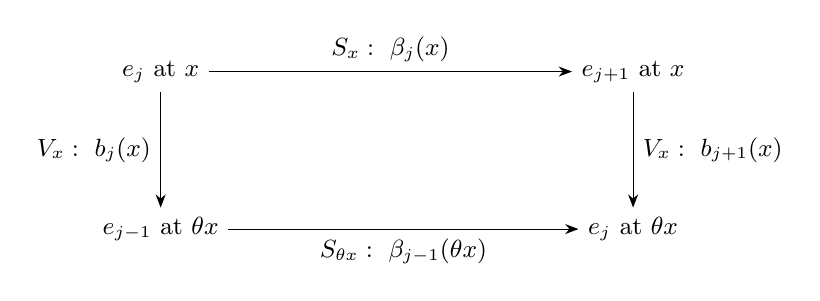
\begin{tikzpicture}[>=Stealth, every node/.style={font=\small}]
\node (a) at (0,2) {$e_j\text{ at }x$};
\node (b) at (6,2) {$e_{j+1}\text{ at }x$};
\node (c) at (0,0) {$e_{j-1}\text{ at }\theta x$};
\node (d) at (6,0) {$e_j\text{ at }\theta x$};
\draw[->] (a)--node[above] {$S_x:\ \beta_j(x)$} (b);
\draw[->] (c)--node[below] {$S_{\theta x}:\ \beta_{j-1}(\theta x)$} (d);
\draw[->] (a)--node[left] {$V_x:\ b_j(x)$} (c);
\draw[->] (b)--node[right] {$V_x:\ b_{j+1}(x)$} (d);
\end{tikzpicture}

\caption{The coefficient identity at a fixed input fiber. Both paths take $e_j$ at $x$ to a multiple of $e_j$ at $\theta x$. The horizontal maps move forward in the coordinate, while the vertical maps move backward and translate the base.}\label{fig:square}
\end{figure}
 We first solve this equation with initial value one, then divide all coefficients in each fiber by a common bound.
For every $x\in X$ set $\widetilde b_0(x)=1$ and define positive coefficients at all integer indices by
\begin{equation}\label{eq:b-recursion}
 \widetilde b_{j+1}(x)
 =\widetilde b_j(x)\frac{\beta_{j-1}(\theta x)}{\beta_j(x)}
 \qquad(j\in\Z).
\end{equation}
Every coefficient is a finite product of positive measurable functions and their reciprocals, so it is finite and measurable.

\begin{lemma}\label{lem:normalization}
For $x\in X_*$, the coefficients $\widetilde b_j(x)$ tend to zero as $j\to+\infty$ and as $j\to-\infty$. Consequently there are measurable functions $b_j:X\to[0,1]$ which are positive on $X_*$ and satisfy
\begin{equation}\label{eq:commuting-coefficients}
 b_{j+1}(x)\beta_j(x)=b_j(x)\beta_{j-1}(\theta x)
 \qquad(x\in X,\ j\in\Z).
\end{equation}
\end{lemma}
\begin{proof}
Taking logarithms in \eqref{eq:b-recursion} and summing forward gives
\begin{align}
 \log\widetilde b_n(x)
 &=\sum_{k=0}^{n-1}\bigl(a_k(x)-a_{k-1}(\theta x)\bigr)\notag\\
 &=-\sum_{k=0}^{n-1}\Delta a_k(x)
       +a_{n-1}(\theta x)-a_{-1}(\theta x),\qquad n\ge1.\label{eq:b-positive}
\end{align}
Summing backward from index $0$ gives the different sign
\begin{align}
 \log\widetilde b_{-q}(x)
 &=-\sum_{k=-q}^{-1}\bigl(a_k(x)-a_{k-1}(\theta x)\bigr)\notag\\
 &=\sum_{k=-q}^{-1}\Delta a_k(x)
       +a_{-q-1}(\theta x)-a_{-1}(\theta x),\qquad q\ge1.\label{eq:b-negative}
\end{align}
Here $a_{-1}=c$. The boundary indices have different forms:
$a_{n-1}=a_{n-1}^+$, whereas $a_{-q-1}=a_q^-$. Using $a_0^\pm=c$ and Equation~\eqref{eq:a-error}, we obtain
\[
 a_{n-1}(\theta x)-c\le c(n-1)+4D(n-1)^{1/3},\qquad
 a_{-q-1}(\theta x)-c\le cq+4Dq^{1/3}.
\]
Combining these bounds with Lemma~\ref{lem:drift}, we obtain the explicit estimates
\begin{align*}
 \log\widetilde b_n(x)&\le -(D-c)n+C(x)-c+4D(n-1)^{1/3},\\
 \log\widetilde b_{-q}(x)&\le -(D-c)q+C(x)+4Dq^{1/3}.
\end{align*}
Since $D-c=90>0$, both right sides tend to $-\infty$. These estimates are pointwise in $x$; they do not require an integrable bound on $C(x)$.

The countable supremum
\[
 L(x)=\sup_{j\in\Z}\widetilde b_j(x)
\]
is measurable, and $1\le L(x)<\infty$ on $X_*$. Define
\[
 b_j(x)=\begin{cases}\widetilde b_j(x)/L(x),&x\in X_*,\\0,&x\notin X_*.
 \end{cases}
\]
All indices at a fixed $x$ are divided by the same number, so \eqref{eq:b-recursion} yields \eqref{eq:commuting-coefficients}. Off $X_*$ both sides of that identity vanish.
\end{proof}

Define a backward shift $V_x:K\to K$ by $V_xe_j=b_j(x)e_{j-1}$. Every $V_x$ has norm at most one, and $x\mapsto V_xv$ is measurable for every $v\in K$ by finite-coordinate approximation. It defines $V\in\B(H_0)$ by
\begin{equation}\label{eq:V-definition}
 (Vf)(\theta x)=V_xf(x),
 \qquad\text{equivalently }(Vf)(\theta x,j-1)=b_j(x)f(x,j).
\end{equation}
Invariance of $\mu$ gives $\norm{Vf}^2=\int_X\norm{V_xf(x)}^2\,d\mu(x)\le\norm{f}^2$.

\begin{proposition}\label{prop:V}
The contraction $V$ commutes with $S$. For every $x\in X_*$ and $h\in\Z$,
\[
 \overline{V_x\Ktail{h}}=\Ktail{h-1},\qquad
 \overline{V_xK}=K.
\]
\end{proposition}
\begin{proof}
At the same output base point $\theta x$, the two compositions have coefficients
\[
 S_{\theta x}V_xe_j=b_j(x)\beta_{j-1}(\theta x)e_j,
 \qquad
 V_xS_xe_j=\beta_j(x)b_{j+1}(x)e_j.
\]
They agree by \eqref{eq:commuting-coefficients}, first on the basis and then on $K$. Equation~\eqref{eq:V-definition} now gives $SV=VS$. On $X_*$ every $b_j(x)>0$. The image of a tail therefore contains every basis vector in the preceding tail, up to a nonzero scalar, and is contained in that preceding tail. This proves the density assertions.
\end{proof}


The density conclusion, rather than surjectivity, is exactly what is needed for closed invariant subspaces. No bounded inverse of $V_x$ or $V$ is asserted.

\section{All common invariant subspaces}\label{sec:subspaces}
We now show that the scalar multipliers, $S$, and $V$ have no proper nonzero closed common invariant subspace. The first step accounts for every closed subspace invariant under the multipliers, without assuming in advance that it is defined fiber by fiber.

\subsection{Multipliers force a measurable field of projections}
Let $M\subseteq H_0$ be a closed subspace invariant under $S$, $V$,
and every scalar multiplier. Since $M_{\bar g}=M_g^*$ belongs to the
same multiplier family, $M$ reduces each multiplier. Its orthogonal
projection $P$ therefore commutes with all of them. The field lemma
\cite[\FieldImportLocator]{CircleCompanion}, applied with the probability
space $(X,\mu)$ and $K=\ell^2(\Z)$, gives
\[
 (Pf)(x)=P_xf(x),\qquad
 M=\{f\in H_0:f(x)\in\ran P_x\text{ for almost every }x\},
\]
where the $P_x$ are orthogonal projections outside one null set and
$x\mapsto P_xv$ is measurable for each $v\in K$. These are exactly the
projection and measurability conclusions needed below; no covariance
property is imposed on this field.

\subsection{Fiber invariance and measurable tail labels}
For this fixed subspace $M$ and its projection field $P_x$, the global invariance identities $(I-P)SP=0$ and $(I-P)VP=0$ imply
\begin{align}
 (I-P_x)S_xP_x&=0,\label{eq:fiber-S}\\
 (I-P_{\theta x})V_xP_x&=0\label{eq:fiber-V}
\end{align}
almost everywhere. To justify the passage, apply each global identity to the constant field $e_j$. In the second identity evaluate the output at $\theta x$ and use probability preservation. The resulting equalities hold for every $j$ on a common conull set and extend to all of $K$ by boundedness. Intersect this set, the projection set, and $X_*$ over all integer iterates of $\theta$. We can henceforth use all these identities on a single invariant conull set. This set is chosen after fixing $M$; no intersection over all candidate subspaces is required.

By Proposition~\ref{prop:fibers} and \eqref{eq:fiber-S}, there is a label
\[
 s(x)\in\Z\cup\{-\infty,+\infty\},\qquad \ran P_x=\Ktail{s(x)}.
\]
It is measurable: for every $j\in\Z$,
\begin{equation}\label{eq:label-measurable}
 \{x:s(x)\le j\}=\{x:\langle P_xe_j,e_j\rangle=1\}
\end{equation}
on the conull set, and the label can be set to $+\infty$ elsewhere. Equation~\eqref{eq:fiber-V} and Proposition~\ref{prop:V} give two implications:
\begin{align}
 s(x)=-\infty&\ \Longrightarrow\ s(\theta x)=-\infty,\label{eq:full-descent}\\
 s(x)\in\Z&\ \Longrightarrow\ s(\theta x)\le s(x)-1.\label{eq:finite-descent}
\end{align}
The first uses $\overline{V_xK}=K$. The second uses $\overline{V_x\Ktail{h}}=\Ktail{h-1}$ and the inclusion $\Ktail{h-1}\subseteq\ran P_{\theta x}$. When the input fiber is zero, there is no restriction on the output label.

\subsection{Strict descent on a probability space}
The final measure argument is useful independently of the construction.
\begin{lemma}\label{lem:descent}
Let $\theta$ be an invertible ergodic probability-preserving transformation of $(Y,\nu)$. Suppose a measurable function $s:Y\to\Z\cup\{-\infty,+\infty\}$ satisfies, almost everywhere,
\[
 s(x)=-\infty\ \Longrightarrow\ s(\theta x)=-\infty,
 \qquad
 s(x)\in\Z\ \Longrightarrow\ s(\theta x)\le s(x)-1.
\]
Then $s=-\infty$ almost everywhere or $s=+\infty$ almost everywhere.
\end{lemma}
\begin{proof}
All inclusions in this proof are modulo null sets. Put $E=\{s=-\infty\}$. The first implication gives $\theta E\subseteq E$. Probability preservation makes this inclusion an equality modulo null sets, so ergodicity gives $\nu(E)\in\{0,1\}$. The case $\nu(E)=1$ is one conclusion.

Suppose $\nu(E)=0$. For each integer $j$, put $F_j=\{s\le j\}$. Both implications give
\[
 \theta F_j\subseteq F_{j-1}\subseteq F_j.
\]
It follows that $\nu(F_{j-1})=\nu(F_j)$. For any fixed $j$, continuity from above now gives
\[
 \nu(F_j)=\nu\left(\bigcap_{r\ge0}F_{j-r}\right)=\nu(E)=0.
\]
The countable union of the $F_j$ is $\{s<+\infty\}$, proving the other conclusion.
\end{proof}

Applying Lemma~\ref{lem:descent} shows that $P_x=I$ almost everywhere or $P_x=0$ almost everywhere. We have therefore proved that the unital complex algebra generated by $S$, $V$, and all scalar multipliers is transitive.

\section{The commutant and structural consequences}\label{sec:structure}
\begin{proof}[Proof of Theorem~\ref{thm:direct-model} and Corollary~\ref{cor:direct-algebra}]
Proposition~\ref{prop:fibers} proves the fiber classification and norm
statement in Theorem~\ref{thm:direct-model}, and
Proposition~\ref{prop:normquasi} gives the uniform power bound and
nonzeroness. Proposition~\ref{prop:V} constructs the commuting
contraction with its dense tail images. Section~\ref{sec:subspaces}
proves transitivity of the algebra generated by $S$, $V$, and the
scalar multipliers. These establish all assertions of the theorem.

That transitive algebra is contained in $\{S\}'$, so any closed
$\{S\}'$-invariant subspace is zero or all of $H_0$. The nonzero
norm-quasinilpotent operator $S$ is nonscalar. The commutant lemma
\cite[\CommutantImportLocator]{CircleCompanion}, with this $S$ on the
complex Hilbert space $H_0$, now implies that $\{S\}'$ is a proper
strongly closed unital complex algebra. Together with the lattice
conclusion, it is transitive.

Finally, the finite residue classes form a countable generating algebra
on $X$, so $L^2(X)$ and $H_0$ are separable. The space $H_0$ is
infinite-dimensional. Every infinite-dimensional separable complex
Hilbert space is unitarily isomorphic to $H_0$; conjugation by such a
unitary transfers $S$, its norm estimates, its commutant, and the
invariant-subspace conclusions. This proves the corollary.
\end{proof}

\subsection{Ordinary invariant subspaces and compactness}
For every $h\in\Z$, the subspace $L^2(X;\Ktail{h})$ is closed,
nonzero, proper, and $S$-invariant. It is not invariant under $V$:
the image of the constant field $e_h$ has its nonzero coordinate at
$h-1$ almost everywhere. Thus the construction separates ordinary
invariance from hyperinvariance in an explicit way.

Each fiber $S_x$ is compact. Indeed $a_k^\pm\ge c(k+1)$ implies
$\beta_j(x)\to0$ as $|j|\to\infty$, and cutting off all but finitely
many shift weights approximates $S_x$ in operator norm. The operator
$S$ on $H_0$ is not compact. There is an infinite orthonormal sequence
$(\varphi_n)$ in $L^2(X)$, since the $N_m$ disjoint residue classes give
$N_m$ orthogonal indicators for every $m$. The orthonormal vectors
$\varphi_n\otimes e_0$ have images
\[
 S(\varphi_n\otimes e_0)=e^{-c}\varphi_n\otimes e_1.
\]
These images are orthogonal with a common positive norm and have no
norm-convergent subsequence.

\subsection{The multiplier algebra has infinite multiplicity}
Let $Q_0$ be the projection onto $L^2(X)\otimes\C e_0$. This gives a
concrete witness to the properness of the commutant: on $1\otimes e_0$,
\[
 Q_0S(1\otimes e_0)=0,\qquad
 SQ_0(1\otimes e_0)=e^{-c}(1\otimes e_1),
\]
so $Q_0\notin\{S\}'$.

The same projection commutes with every scalar multiplier, but is not
itself a scalar multiplier. If $Q_0=M_g$, its action on $1\otimes e_0$
would give $g=1$ almost everywhere, whereas its action on
$1\otimes e_1$ is zero. The abelian self-adjoint algebra
$\{M_g:g\in L^\infty(X)\}$ is therefore not maximal abelian in
$\B(H_0)$. Arveson's maximal-abelian inclusion theorem
\cite[Theorem~3.3]{Arveson1967} does not apply to this subalgebra of the
transitive commutant.

\subsection{Atomic finite families and a diffuse joint algebra}
We finish with a spectral property of the constructed weights. This
subsection is independent of the transitivity proof.

Let $|S|=(S^*S)^{1/2}$. Identify $H_0$ with
$L^2(X\times\Z,\mu\times\#)$, where $\#$ is counting measure,
and let $Ue_j=e_{j+1}$ on every fiber. Then
\[
 S=U|S|,\qquad (|S|f)(x,j)=\beta_j(x)f(x,j).
\]
All weights are positive, so $|S|$ is injective with dense range and
$U$ is the unitary polar part of $S$. Define
\[
 A_n=U^{-n}|S|U^n\quad(n\in\Z);
 \qquad (A_nf)(x,j)=\beta_{j+n}(x)f(x,j).
\]
For a family of operators, $W^*$ denotes the smallest strongly closed
unital self-adjoint algebra containing that family. A nonzero projection
in an abelian von Neumann algebra is minimal if it contains no smaller
nonzero projection in that algebra. Such an algebra is \emph{atomic}
when its identity is the strong sum of its minimal projections, and
\emph{diffuse} when it has no minimal projection. We will show that
$W^*(A_n:n\in F)$ is atomic for every finite $F\subset\Z$, whereas
$W^*(A_n:n\in\Z)$ is diffuse.

For any finite $F\subset\Z$ and fixed $j$, the tuple
$(\beta_{j+n}(x))_{n\in F}$ depends on finitely many residues $T_m(x)$.
Because the residues are nested, it depends on one residue $T_M(x)$
and takes finitely many values. Allowing the countably many values of
$j$ gives a countable range for the joint tuple on $X\times\Z$.
Its nonempty level sets have positive measure: on every fixed coordinate
slice they are finite unions of residue classes. These level sets give
the minimal projections of the generated abelian algebra, and their
sum is the identity. Thus $W^*(A_n:n\in F)$ is atomic. In particular,
$|S|$ has a pure-point spectral resolution.

For the full family, the two equal central weights determine the
coordinate slice. They are the only weights equal to $e^{-c}$, since
$a_k^\pm\ge c(k+1)>c$ for every $k\ge1$. At $(x,j)$ the tuple indices
$n$ for which $\beta_{j+n}(x)=e^{-c}$ are therefore exactly
$-j-1$ and $-j$. For every $r\in\Z$, the projection onto the slice
$j=r$, denoted by $P_r$, belongs to $W^*(A_n:n\in\Z)$: it is
\[
 \mathbf1_{\{e^{-c}\}}(A_{-r-1})\,
 \mathbf1_{\{e^{-c}\}}(A_{-r}).
\]
Next fix $m\ge1$ and choose $k_m=\ell_{m-1}\in I_m$. On the slice
$j=r$, the multiplier $A_{k_m-r}$ supplies $\beta_{k_m}(x)$.
For $0\le t<N_m$, put
\[
 \lambda_{m,t}=\exp[-c(k_m+1)-J_m-Dt].
\]
Equation~\eqref{eq:a-plus} shows that the multiplication projection
of the residue rectangle $\{T_m=t\}\times\{r\}$ is
\[
 P_r\,\mathbf1_{\{\lambda_{m,t}\}}(A_{k_m-r}).
\]
Thus every residue-class projection on every coordinate slice belongs
to the generated algebra. Such rectangles generate the product
sigma-algebra. Conversely all $A_n$ are multiplication operators, so,
modulo completion and null sets,
\[
 W^*(A_n:n\in\Z)
   =L^\infty(X\times\Z,\mu\times\#)
\]
in its multiplication representation. Haar measure on $\Z_2$ has no
atoms, and consequently this algebra is diffuse.

The pure-point assertion does not assert discreteness of the spectrum
or compactness of $S$. Nor is this full multiplier algebra the scalar
base algebra used in the transitivity proof. In fact $|S|$ does not
commute with $S$, because the adjacent weights $\beta_0=e^{-c}$ and
$\beta_1\le e^{-2c}$ differ. The polar-conjugate algebra is therefore
not contained in $\{S\}'$.

\bibliographystyle{plain}
\bibliography{references}
\end{document}
